%% -*- coding: utf-8-unix -*-

\chapter{テストシナリオ実装}
\label{chap:poc-scenario-dev}

 \section{テストシナリオの概要}

  \subsection{ネットワークテストの方針}

\ref{chap:poc-target-design}章で設定したとおり、\yo ネットワークのテスト
を考える。そのためのテストシナリオとして「静的なふるまいのテスト」「動的
なふるまいのテスト」の2種類を実装する。テストシナリオ実装・テスト実行を
通して、物理ネットワークのテスト自動実行のポイント検討や問題点の抽出、従
来の人手によるテスト作業との比較を行なう。

  \subsection{BDDテストシナリオの基礎}
  % - TDD/BDDとBDDツールとしてのCucumber
  % - Narrative
  % - ネットワークテストを書く上での検討点、今回のプロジェクトでの方針・決めごと
  %   - なぜそうきめたのか?

      \paragraph{テストツール}
NetTesterはテスト用ノードの生成・テスト対象ネットワークへの配置(パッチ接
続)をおこなうためのAPIを提供する。提供されるAPIを使用して \yo ネットワー
クのテストを実装する。\footnote{実際に作成した自動テストのためのコードは
NetTester Examples~\cite{nettester-ex}として公開している。}

テストシナリオの記述については、アプリケーションのテストでつかわれる既存
のツールと連携することを想定している。本PoCでは、「BDDによるネットワーク
のテスト」を考えていること(\ref{sec:behavior-test}節)、広く使われている
ツールであること、RubyベースでNetTesterとの親和性が高いことをもとに、BDD
ツールであるCucumber\footnote{Cucumber \url{https://cucumber.io/}}を採用
した。

    \paragraph{Narrative}
    % Cucumber の .feature の書き方 – NetTester
    %   https://3.basecamp.com/3088280/buckets/867009/messages/155991347
    % クライアントの要望にこたえるWebサービス開発 ~「らせん型ワークフロー」のススメ~
    %  http://www.slideshare.net/mayuco/css-nite-in-sapporo-vol5-14085124
BDDでは、テストのストーリー(フィーチャ)を以下のような構造で記述する
\cite{rspec-book,spiral-workflow}。
\begin{description}
 \item[タイトル] どのストーリーについて説明するのかを示す。タイトルは一
            般に、ユーザがシステムに要求するかもしれないアクティビティを
            短い言葉で表したものになる。
 \item[ナラティブ] ストーリーの内容について説明をする。一般的には
            Connextraフォーマットと呼ばれる形式の短い文章で記述される。
            このテンプレートは、誰がシステムを使っていて、そのユーザは何
            をしていて、なぜそのことに関心があるのか、を明確にする。
            \begin{itemize}
             \item ``As a (role)'': [誰のために(role)]として
             \item ``I want (feature)'': [何を(feature)]したい
             \item ``So that (bussiness value)'': なぜなら[なぜ
                   (bussiness value)の]ためだ
            \end{itemize}
 \item[受け入れ基準] ストーリーの完了・完成を定義する受け入れ基準、シナ
            リオの定義。
\end{description}

Cucumberにおけるフィーチャとは、システムを利用するユーザーまたは別のコン
ピュータの視点に立っておおまかに表現された要件のことを指す。Cucumberの
フィーチャはタイトルと簡単なナラティブ、受け入れ基準としての役割をはたす
自動化されたシナリオによって構成される。
\begin{itemize}
 \item フィーチャはタイトルとナラティブで構成され複数のシナリオを含む。
       (本プロジェクトでは\verb|features/*.feature|ファイル)
       \begin{itemize}
        \item シナリオはそれぞれ、シナリオ内でおこることを任意のステップ
              で記述する。
       \end{itemize}
 \item 個々のステップ定義は開発で使っているシステムの言語で記述される。
       (本プロジェクトではRuby: \verb|features/step_definitions/*.rb|ファ
       イル)
\end{itemize}

% Narrative を Pull Requst する – NetTester
%   https://3.basecamp.com/3088280/buckets/867009/todos/159223633
% NetTester機能拡張(NW機器間接続)方針・やりたいこと – NetTester
%   https://3.basecamp.com/3088280/buckets/867009/todos/182746431
% Firewall の cucumber シナリオ – NetTester
%   https://3.basecamp.com/3088280/buckets/867009/todos/158299550

\subsection{静的なテストの実装}
テストシナリオ策定の考えかた…そもそもなにをするテストなのか。どのような
検討を経てテストシナリオをきめたのか。narrativeの定義のプロセスとか。

OOD資料にかいたようなテストコード解説のはなしをこちらにも含めるか?
\begin{itemize}
 \item 実装
       \begin{itemize}
        \item Step2テスト業務で気づいたことをまとめる – NetTester \url{https://3.basecamp.com/3088280/buckets/867009/todos/260220903}
       \end{itemize}
\end{itemize}

\subsection{動的なテストの実装}

% 障害試験シナリオを書く – NetTester
% \url{https://3.basecamp.com/3088280/buckets/867009/todos/238169066}

PoC環境(詳細は\figref{fig:poc-env-physical-detail})では
\figref{fig:poc-env-linkdown}のようにtester set 1を「動的なふるまいのテ
スト」用に使用するよう設計している。PoCでは、\yo 内部ネットワークの中心
となるFWの冗長化機能試験をおこなう。そのため、テストシナリオではFWの
Active/Passive切替トリガとなるActive側(FW1)リンクダウン/リンクアップ操作
を実装する。物理リンク操作のため物理OpenFlowスイッチ(OFS1)へ以下の2リン
クをそれぞれ引き込んでいる。
\begin{itemize}
 \item L3SW-FW1 間リンク (FW1 Uplink)
 \item FW1-L2SW1 間リンク (FW1 Downlink)
\end{itemize}

\begin{figure}[h]
 \centering
 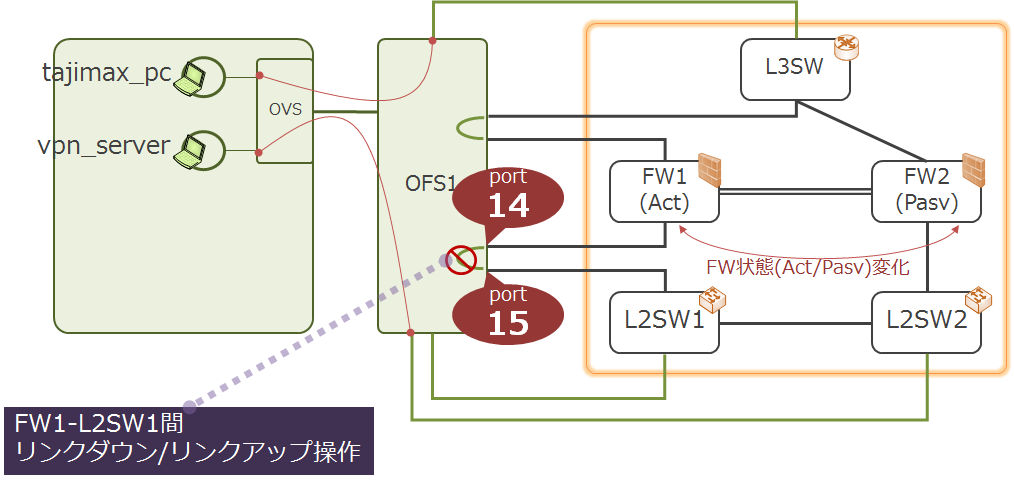
\includegraphics[scale=0.6]{img/poc-env-linkdown.png}
 \caption{PoC環境: NetTesterによるリンクダウン操作}
 \label{fig:poc-env-linkdown}
\end{figure}

\section{テストシナリオ実装における検討ポイント}

\subsection{Teardown処理}

\begin{itemize}
 \item Target network の状態
       \begin{itemize}
        \item ARP Table のクリア
        \item NAT Table のクリア
        \item Firewall の active/standby (自動復旧にしているのでとくにいれていない)
       \end{itemize}
 \item Netns の /etc 配下のクリア
       \begin{itemize}
        \item 自作echoサーバーで通信開始時に10秒のラグが起きる問題 – NetTester \url{https://3.basecamp.com/3088280/buckets/867009/todos/274457003}
       \end{itemize}
 \item 物理OFSのflow tableのクリア (まだやれてない)
\end{itemize}

\subsection{テストシナリオのサイズ}

シナリオサイズの目安、シナリオ分割の目安 (step3 test つくっているときに
分割するって話になった理由は?)

\subsection{ステップ実装上の工夫}
\begin{itemize}
 \item ニセ○○サーバとステップ実装 – NetTester \url{https://3.basecamp.com/3088280/buckets/867009/documents/216490375}
 \item コマンドをバックグラウンド実行 – NetTester \url{https://3.basecamp.com/3088280/buckets/867009/documents/216399643}
 \item step内でのバックグラウンドコマンド実行 – NetTester \url{https://3.basecamp.com/3088280/buckets/867009/todos/202691188}
 \item factory\_girl で仮想ホストを作る – NetTester \url{https://3.basecamp.com/3088280/buckets/867009/documents/210831650}
\end{itemize}

\section{PoCの結果と評価}

\subsection{実際に発見できた問題点}
テストとしての結果まとめ
\begin{itemize}
  \item 結果: 実際に発見できたトラブルや設定ミスなどをあげる。
       \begin{itemize}
        \item Teardown関連
              \begin{itemize}
               \item 原因切り分けメモ (muraki) – NetTester \url{https://3.basecamp.com/3088280/buckets/867009/documents/217782147}
               \item 調査: テスト環境でシナリオ実行すると2回目以降でコケる – NetTester \url{https://3.basecamp.com/3088280/buckets/867009/todos/218486066}
              \end{itemize}
        \item Target Network の設定不備の発見
              \begin{itemize}
               \item DNSのテスト作る – NetTester \url{https://3.basecamp.com/3088280/buckets/867009/todos/301325453}
               \item 通信要件\#10 A社内PC→インターネットの疎通確認(ICMP) – NetTester \url{https://3.basecamp.com/3088280/buckets/867009/todos/233175867}
               \item 通信要件\#29 B社PC→DMZ内のVPNサーバの疎通確認(SSLVPN) – NetTester \url{https://3.basecamp.com/3088280/buckets/867009/todos/233178490}
              \end{itemize}
       \end{itemize}
\end{itemize}

step3
\begin{itemize}
 \item 実装 (NAT IPの変更とかデモの話をどこまで含めるか?)
 \item 結果
\end{itemize}

\subsection{ネットワークの構築・運用プロセスに対する定性的な評価}
評価・考察
\begin{itemize}
 \item テスト実装のコスト
 \item 繰り返し実行できることのメリット
       \begin{itemize}
        \item OSの更新などおおきな変更にたいするリスクヘッジ
       \end{itemize}
\end{itemize}


%%% Local Variables:
%%% mode: yatex
%%% TeX-master: "main.tex"
%%% End:
